\documentclass[tikz,border=10pt]{standalone}%[12pt]{article}
\usepackage{tikz}
\usetikzlibrary{shadows,arrows,shapes,positioning,calc}

\tikzset{
ell/.style={draw,fill=blue!10,fill opacity=0.3,ellipse,minimum height=2em,minimum width=0.5*#1cm,align=right},
line/.style={-,line width=0.5pt},
dot/.style = {draw,fill,circle,inner sep=0pt,outer sep=0pt,minimum size=2pt},
}
\begin{document}

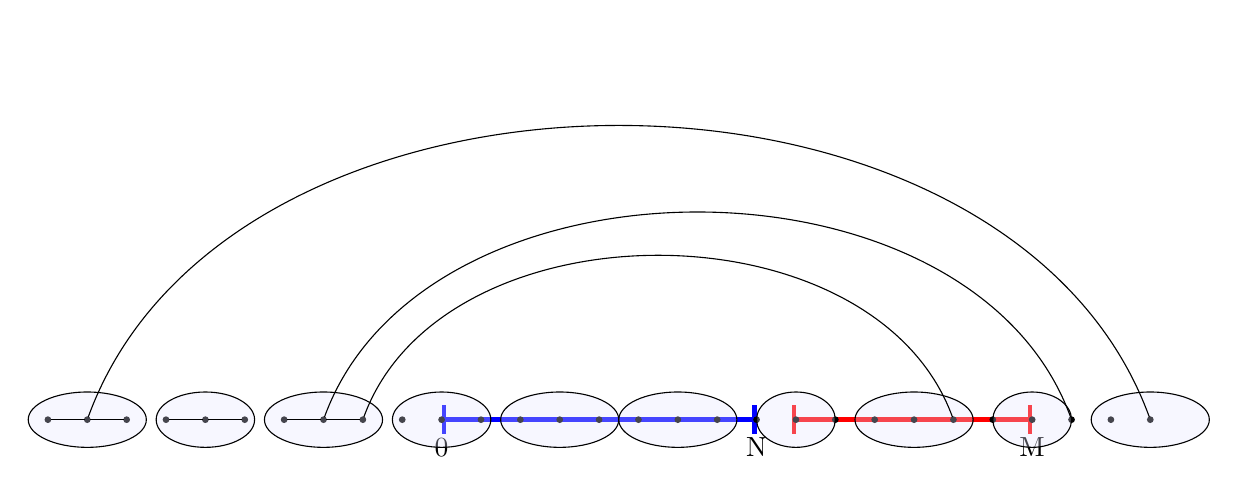
\begin{tikzpicture}[scale=0.5]
  \draw[blue,ultra thick,|-|] (0,0) -- (8,0);
  \draw (0,-2em) node {0} (8,-2em) node {N} (15,-2em) node {M};

  \draw[red,ultra thick,|-|] (8.9,0) -- (15,0);
  \draw foreach \i in {-10,...,18} {(\i,0) node[dot] (n\i) {}};
  \draw foreach \i/\w in {-3/3,-2/2.5,-1/3,0/2.5,1/3,2/3,3/2,4/3,5/2,6/3}
  { (\i*3,0) node[ell=\w] (c\i) {} };
  \draw (n-10) -- (n-9) -- (n-8)
  (n-7) -- (n-6) -- (n-5)
  (n-4) -- (n-3) -- (n-2);
  \draw (n-3) edge[out=70,in=110] (n16);
  \draw (n-2) edge[out=70,in=110] (n13);
  \draw (n-9) edge[out=70,in=110] (n18);
\end{tikzpicture}


\end{document}

